% 2009 年安徽卷理科第 18 题：四棱锥 F-ABCD 与四棱锥 E-ABCD 共底。
% 来源 PDF：普通高考/2009/2009安徽理.pdf，SHA256 e3986483e52654337c383d27cbe67e80ee0bd62eaf64defba6fe8bcc0cdb0c6d
% 原页：第 2 页（A3 三栏）第 1 栏上部，印刷页 496。
% 重绘依据：按原图菱形 ABCD 以斜投影画出，A 在左、D 在前下、C 在右、B 在后方（被遮挡）；
%   E 在 A 正上方、F 在 C 正上方，AE、CF 竖直；FA、FD、FC 与 AD、DC 实线，
%   AB、BC、BF 因被遮挡画虚线。
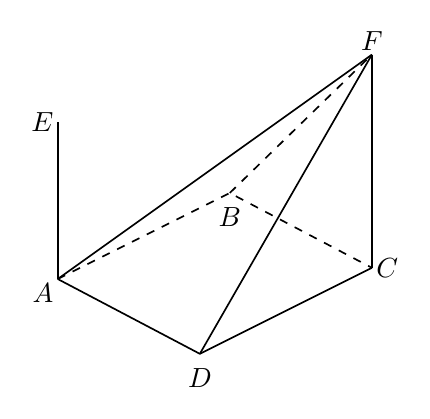
\begin{tikzpicture}[scale=0.95, semithick, every node/.style={inner sep=1.3pt}]
  \coordinate (A) at (0,0);
  \coordinate (D) at (1.9,-1.0);
  \coordinate (C) at (4.2,0.15);
  \coordinate (B) at (2.3,1.15);
  \coordinate (E) at (0,2.1);
  \coordinate (F) at (4.2,3.0);
  % 底面
  \draw (A) -- (D) -- (C);
  \draw[dashed] (A) -- (B) -- (C);
  % 侧棱
  \draw (A) -- (F);
  \draw (D) -- (F);
  \draw (C) -- (F);
  \draw[dashed] (B) -- (F);
  % 竖直棱
  \draw (A) -- (E);
  \node[below left] at (A) {$A$};
  \node[below] at ([yshift=-4pt]D) {$D$};
  \node[right] at (C) {$C$};
  \node[anchor=north] at ([yshift=-4pt]B) {$B$};
  \node[left] at (E) {$E$};
  \node[above] at (F) {$F$};
\end{tikzpicture}
